% Asset ID: A22StatisticalHypothesisTestingTikZ-002
% Source: Chapter 7 Hypothesis Testing Binomial transcript
% Related lesson section: Worked Example 1
% Purpose: Show the prize-game lower-tailed test.
% Related LO IDs: A22-HT-LO001, A22-HT-LO002, A22-HT-LO003

\documentclass[tikz,border=8pt]{standalone}
\usepackage{amsmath}
\usetikzlibrary{arrows.meta, positioning, decorations.pathreplacing}
\begin{document}
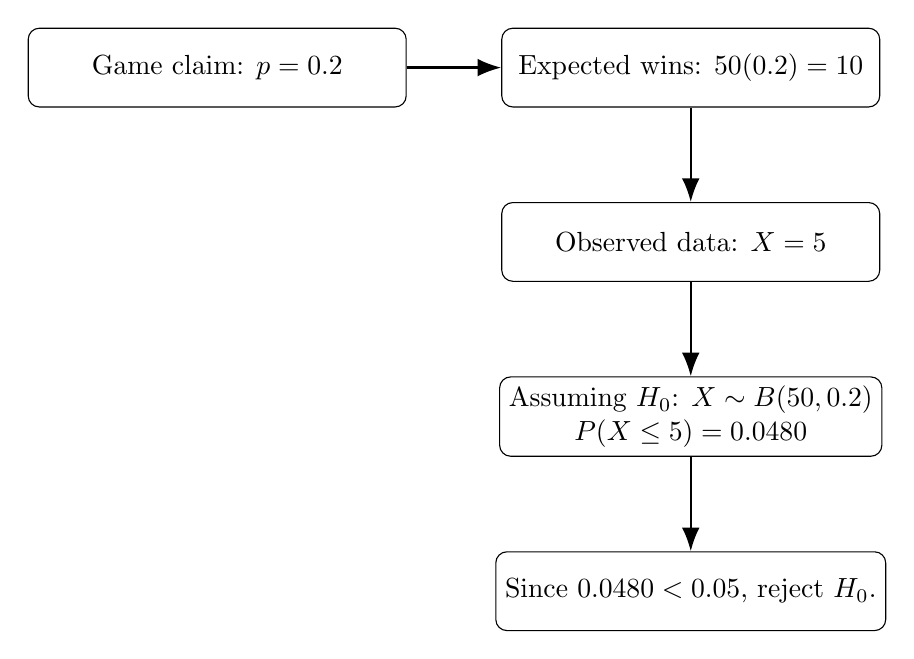
\begin{tikzpicture}[node distance=1.2cm, box/.style={draw, rounded corners, align=center, minimum width=4.8cm, minimum height=1.0cm}, arrow/.style={-{Latex[length=3mm]}, thick}]

\node[box] (claim) {Game claim: \(p=0.2\)};
\node[box, right=of claim] (expected) {Expected wins: \(50(0.2)=10\)};
\node[box, below=of expected] (observed) {Observed data: \(X=5\)};
\node[box, below=of observed] (prob) {Assuming \(H_0\): \(X\sim B(50,0.2)\)\\\(P(X\leq 5)=0.0480\)};
\node[box, below=of prob] (conc) {Since \(0.0480<0.05\), reject \(H_0\).};
\draw[arrow](claim)--(expected);\draw[arrow](expected)--(observed);\draw[arrow](observed)--(prob);\draw[arrow](prob)--(conc);

\end{tikzpicture}
\end{document}
